\documentclass[landscape,headrule,footrule]{foils}
\usepackage{foilenv}
\usepackage{mathrsfs}
\usepackage{amsfonts}

\begin{document}

\title       {Banach Wessenstian GAN
\footnote{Jonas Adler, KTH-Royal institute of Technology Research and Physics \\
Sebastian Lunz, University of Cambridge}
\\[12pt]
\normalsize NeurIPS 2018}

\author      {\large Sheng-Je Huang \\[1em]
              Institute of Communications Engineering \\
              National Chiao Tung University, Hsinchu}
\date        {Feburary 20 , 2019}
\MyLogo      {}
\Restriction {}
\rightfooter {\thepage}
\rightheader {\hyperlink{toc}{top~$\blacktriangle$}}
\leftheader  {}
\maketitle
\tableofcontents
%----------------------------------------------------------%
\section{Introduction}
\tableofcontents

\begin{frame}[\secname]
\begin{center}
\begin{itemize}
\item Extend WGAN implemented via a \textbf{gradient penalty} (GP) term to any separable complete normed space. \\
\item Efficiently implemented BWGAN by replacing the $\ell^{2}$ norm into \textbf{dual norm}. \\
\item Give theoretically grounded heuristics for the choice of regularization parameters. \\
\end{itemize}
\end{center}
\end{frame}

%-----------------------------------------------------------%
\section{Background}
\subsection{Generative adversarial networks}
\tableofcontents
\begin{frame}[Generative adversarial networks]
\begin{flushleft}
\begin{itemize}
\item GANs perform generative modeling by learning a map $G : Z\rightarrow B$ from a low-dimensional \textbf{latent space $Z$} to \textbf{image space $B$}, mapping a fixed noise distribution $\mathbb{P}_{Z}$ to a distribution of generated images $\mathbb{P}_{G}$. \\
\item The famous \textbf{minimax} game between generator $G$ and critic $D$
\begin{equation}
\mathop{\min}_{G} \mathop{\max}_{D} \mathbb{E}_{X\thicksim\mathbb{P}_{r}} [\log (D(x))]+ \mathbb{E}_{Z\thicksim\mathbb{P}_{Z}}[\log (1-D(G_{\Theta}(Z)))].
\end{equation}
\\
\item Using \textbf{Jensen-Shannon divergence} as distance measure between the dirstirbutions $\mathbb{P}_{G}$ and $\mathbb{P}_{r}$.
\end{itemize}
\end{flushleft}
\end{frame}

%-----------------------------------------------------------%
\subsection{Wasserstein metrics}
\tableofcontents
\begin{frame}[Wasserstein metrics (1/2)]
\begin{flushleft}
\begin{itemize}
\item To overcome undesirable behavior of the JSD in the presence of \textbf{singular measures}, using the Wasserstein metric to quantify the distance between the distributions $\mathbb{P}_{G}$ and $\mathbb{P}_{r}$. \\
\item The Wasserstein distance provide \textbf{meaningful gradients} to the gernerator even when the measures are mutually singular. \\
\item The Wasserstein-$p$, $p\geqq 1$, distance is defined as
\begin{equation}
{\rm Wass}_p(\mathbb{P}_{G},\mathbb{P}_{r}):= \left(\mathop{\inf}_{\pi\in\Pi(\mathbb{P}_{G}, \mathbb{P}_{r})} \mathbb{E}_{(X_1,X_2)\thicksim \pi} d_B(X_1,X_2)^p \right)^{1/p}
\end{equation}

\end{itemize}
\end{flushleft}
\end{frame}

%-----------------------------------------------------------%
\begin{frame}[Wasserstein metrics (2/2)]
\begin{flushleft}
\begin{itemize}
\item The infimum is highly intractable.\\
\item The \textbf{Kantorovich-Rubinstein duality} provides a way of more efficiently computing the Wasserstein-1 distance.
\begin{equation}
{\rm Wass}_p(\mathbb{P}_{G},\mathbb{P}_{r})= \mathop{\sup}_{{\rm Lip}(f)\leq 1} \mathbb{E}_{X\thicksim \mathbb{P}_{G}}f(X)- \mathbb{E}_{X\thicksim \mathbb{P}_{r}}f(X)
\end{equation}
\\
\item The supremum is taken over all Lipschitz continuous functions $f:B\rightarrow \mathbb{R}$ with Lipschitz constant equal or less than one.\\
\item If we consider $\gamma$-Lipschitz with a function $f:B\rightarrow \mathbb{R}$, we can get
\begin{center}
	$|f(x)-f(y)| \leq \gamma d_B(x,y)$.
\end{center}
\end{itemize}
\end{flushleft}
\end{frame}

%-----------------------------------------------------------%

\begin{frame}[Wasserstein metrics]
\begin{flushleft}
\begin{itemize}
\begin{figure}
\center
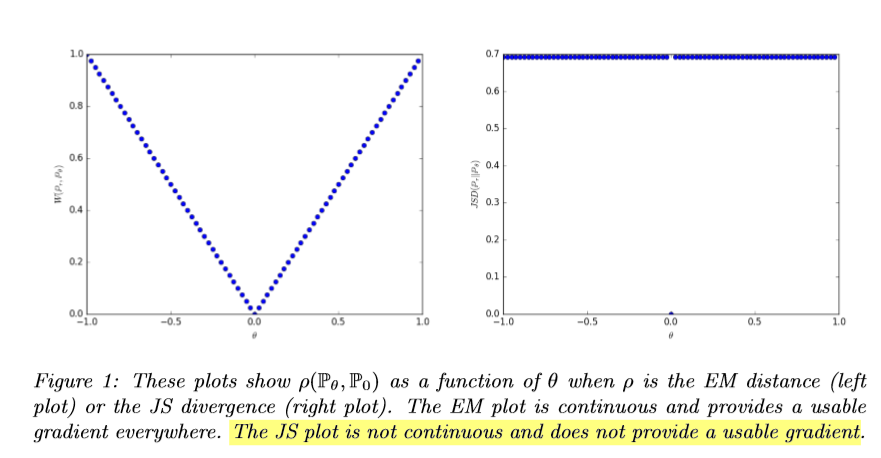
\includegraphics[scale=0.8]{figure/fig_wgan.png}
\end{figure}

\end{itemize}
\end{flushleft}
\end{frame}

%-----------------------------------------------------------%
\subsection{Wasserstein GAN}
\tableofcontents
\begin{frame}[Wasserstein GAN]
\begin{flushleft}
\begin{itemize}
\item Implementing GANs with the Wasserstein metric requires to approximate the supremum in (3) with a neural network.
\\
\item Original WGAN \footnote{Martin Arjovsky, Soumith Chintala, and Leon Boeou. Wasserstein Generative Adversarial Networks.\textit{International Conference on Machine Learning,} \textsl{ICML}, 2017} using \textbf{weight clipping} to statisfy the Lipschitz constraint.
\\
\item However weight clipping in WGAN leads to optimization difficulties, and that even when optimization succeeds the resulting critic can have a pathological value surface.
\end{itemize}
\end{flushleft}
\end{frame}

%-----------------------------------------------------------%
\subsection{Improved Wasserstein GAN}
\tableofcontents
\begin{frame}[Improved Wasserstein GAN \footnote{Ishaan Gulrajani, Faruk Ahmed, Martin Arjovsky, Vincent Dumoulin, and Aaron C Courville. Improved training of wasserstein gans. \textit{Advances in Neural information Processing Systems} \textsl{(NIPS)}, 2017.}]
\begin{flushleft}
\begin{itemize}
\item \textbf{Gradient penalty} as an uncontrollable additional constraint becomes another characterization of 1-Lipschitz functions.
\\
\item In particular, they prove that if $B=\mathbb{R}^n, d(x,y)_B=\Vert x-y \Vert_2$ we have the gradient characterization
\begin{center}
	$f$ is 1-Lipschitz $\Longleftrightarrow \Vert \nabla f(x) \Vert_2 \leq 1$ for all $x\in \mathbb{R}^n$. \\
\end{center}	
\item Penalty term to the \textbf{loss function} of $D$ that takes the form
\begin{equation}
\mathbb{E}_{\widehat{X}} \left( \Vert \nabla D(\widehat{X}) \Vert_2 -1 \right)^2
\end{equation}
\end{itemize}
\end{flushleft}
\end{frame}

%-----------------------------------------------------------%
\subsection{Banach spaces}
\tableofcontents
\begin{frame}[Banach spaces (1/3)]
\begin{flushleft}
\begin{itemize}
\item We often choose the $\ell^2$ norm as underlying distance measure on \textbf{image space}, but many other distance notions are possible that account for more specific image features.
\\
\item If a vector space $B$ is equipped with a notion of \textbf{length}, a norm $\Vert \cdot \Vert_B :B\rightarrow \mathbb{R}$, we call it a \textbf{normed space}.
\\
\item A normed space is called a \textbf{Banach space} if it is complete, that is, Cauchy sequences converge.
\\
\item All separable Banach spaces are Polish spaces and we can define Wasserstein metrics on them using the induced metric $d_B (x,y)= \Vert x-y \Vert_B$.
\end{itemize}
\end{flushleft}
\end{frame}

%-----------------------------------------------------------%
\begin{frame}[Banach spaces (2/3)]
\begin{flushleft}
\begin{itemize}
\item For any Banach space B, we can consider the space of all bounded linear functionals $B \rightarrow \mathbb{R}$, which we will denote $B^*$ and call the \textbf{topological dual of $B$}.
\\
\item Banach space with norm $\Vert \cdot \Vert_{B^*} :B^* \rightarrow \mathbb{R}$ given by 
\begin{equation}
\Vert x^* \Vert_{B^*} = \mathop{\sup}_{x \in B} \dfrac{x^*(x)}{\Vert x \Vert_B}.
\end{equation}
\end{itemize}
\end{flushleft}
\end{frame}

%-----------------------------------------------------------%
\begin{frame}[Banach spaces (3/3)]
\begin{flushleft}
The set of functions $x:\Omega \rightarrow \mathbb{R}$ with \textbf{norm}
\begin{itemize}
\item \textbf{$L^p$-spaces:} 
\begin{equation}
\Vert x \Vert_{L^p} = \left( \int_{\Omega} x(t)^p dt \right)^{1/p}
\end{equation}
\\
is a Banach with dual $[L^p]^* = L^q$ where $1/p + 1/q = 1$.
\\
\item \textbf{Sobolev spaces:}
\begin{equation}
\Vert x \Vert_{W^{1,2}} = \left( \int_{\Omega} x(t)^2 + |\nabla x(t)|^2 dt \right)^{1/2}
\end{equation}
\\
It can rewrite the equation by multiplying with $\xi$ in the Fourier space
\begin{equation}
\Vert x \Vert_{W^{s,p}} = \left( \int_{\Omega} \left( \mathcal{F}^{-1} \left[(1+| \xi |^2)^{s/2} \mathcal{F}x \right] (t) \right)^p dt \right)^{1/p}.
\end{equation}
\end{itemize}
\end{flushleft}
\end{frame}

%-----------------------------------------------------------%
\section{Banach Wasserstein GANs}
\tableofcontents
\begin{frame}[Banach Wasserstein GANs]
\begin{flushleft}
\begin{itemize}
\item In particular, for any Banach space $B$ with norm $ \Vert\cdot\Vert_B$, we will derive the loss function
\begin{equation}
L = \dfrac{1}{\gamma} (\mathbb{E}_{X \sim \mathbb{P}_{\theta}} D(X)-\mathbb{E}_{X \sim \mathbb{P}_{r}} D(X)) + \lambda \mathbb{E}_{\hat{X}} \left(\dfrac{1}{\gamma} \textcolor{red}{\Vert \partial D(\hat{X}) \Vert_{B^*}} - 1 \right)^2
\end{equation}
where $\lambda,\gamma \in \mathbb{R}$ are \textbf{regularization parameters}.
\end{itemize}
\end{flushleft}
\end{frame}

%-----------------------------------------------------------%
\subsection{Enforcing the Lipschitz constraint}
\tableofcontents
\begin{frame}[Enforcing the Lipschitz constraint (1/3)]
\begin{flushleft}
\begin{itemize}
\item We require a more \textbf{general notion of gradient}: \\
The function $f$ is call \textit{Fréchet differentiable} at $x \in B$ if there is a bounded linear map $\partial f(x) :B \rightarrow \mathbb{R}$ such that
\begin{equation}
\mathop{\lim}_{\Vert h \Vert_B \rightarrow 0} \dfrac{1}{\Vert h \Vert_B} |f(x+h) - f(x) - [\partial f(x)] (h)| = 0.
\end{equation}
\item The gradient $\nabla f(x)$ in $\mathbb{R}^n$ with the standard inner product is connected to  the Fréchet derivative via $[\partial f(x)](h) = \nabla f(x) \cdot h$.
\\
\end{itemize}
\end{flushleft}
\end{frame}

%-----------------------------------------------------------%
\begin{frame}[Enforcing the Lipschitz constraint (2/3)]
\begin{flushleft}
\begin{itemize}
\item \textbf{Lemma 1}
\textit{Assume $f:B \rightarrow \mathbb{R}$ is Fréchet differentiable. Then $f$ is $\gamma$-Lipschitz if and only if} \\
\begin{equation}
\Vert \partial f(x) \Vert_{B^*} \leq \gamma \quad \forall x \in B.
\end{equation}
 \\
\item According to the \textbf{Lemma 1}, we can get the \textit{$\gamma$-Lipschitz contraints} \\
\begin{center}
$|f(x) - f(y)| \leq \gamma \Vert x-y \Vert_B$ \\
\end{center}
\end{itemize}
\end{flushleft}
\end{frame}

%-----------------------------------------------------------%
\begin{frame}[Enforcing the Lipschitz constraint (3/3)]
\begin{flushleft}
\begin{itemize}
\item Gradient norm penalization requires characterizing the dual $B^*$ of $B$. In a \textbf{finite dimension}, there is an linear continuous bijection $\iota: \mathbb{R}^n \rightarrow B$ given by
\begin{equation}
\iota(x)_i = x_i.
\end{equation}
%\item Although this does not generalize to the infinite dimensional setting, we hope that this is not a very limiting assumption in practice. \\
\item We can write $f = g\circ \iota$  where $g: \mathbb{R}^n \rightarrow \mathbb{R}$ and we can get  $ \partial f(x) = \iota^* (\partial g(\iota(x)))$ by the \textbf{chain rule}.
($\iota^* :\mathbb{R}^n \rightarrow B^*$ is the adjoint of $\iota$.) \\
\item The derivative in \textbf{finite dimensional Banach spaces} can be done using standard automatic differentiation libraries. \\

\end{itemize}
\end{flushleft}
\end{frame}

%-----------------------------------------------------------%
\subsection{Regularization parameter}
\tableofcontents
\begin{frame}[Regularization parameter (1/2)]
\begin{flushleft}
\begin{itemize}
\item Regularization term:
\begin{center}
$ \textcolor{red}{\lambda} \mathbb{E}_{\hat{X}} \left(\dfrac{1}{\textcolor{red}{\gamma}} \Vert \partial D(\hat{X})\Vert_{B^*} - 1 \right)^2$. \\
\end{center}
\item In order to avoid having to hand-tune parameters for every choice of norm, author derive some \textbf{heuristic parameter} choice rules. \\
\item Assuming that $G$ is the zero-generator and symmetry of $\mathbb{P}_r$, the $D$ will be decided by a single constant $f(x) = c \Vert x \Vert_B$. \\
We can form the optimization problem
\begin{center}
$\mathop{\min}_{c \in \mathbb{R}} \mathbb{E}_{X \sim \mathbb{P}_r} \left[-\dfrac{c \Vert X \Vert_B}{\gamma} + \dfrac{\lambda(c- \gamma)^2}{\gamma^2} \right]$.
\end{center}

\end{itemize}
\end{flushleft}
\end{frame}

%-----------------------------------------------------------%
\begin{frame}[Regularization parameter (2/2)]
\begin{flushleft}
\begin{itemize}
\item By solving optimization problem, we can obtain \\
\begin{center}
$c = \gamma \left(1+\dfrac{\mathbb{E}_{X \sim \mathbb{P}_r} \Vert X \Vert_B}{2 \lambda} \right)$. \\
\end{center}
\item Since the norm has Lipschitz constant 1, we want $c\approx \gamma$. To has a small relative error, we get the heuristic rule
\begin{center}
$ \lambda \approx \mathbb{E}_{X \sim \mathbb{P}_r} \Vert X \Vert_B$. \\
\end{center}
\item 
Assuming $\lambda$ was appropriately chosen, we find in general (by lemma 1) $\Vert \partial D(x) \Vert_{B^*} \approx \gamma$. We want to enforce $\Vert x \Vert_{B^*} \approx \Vert \partial D(x) \Vert_{B^*}$, hence $\gamma \approx \Vert x \Vert_{B^*}$. \\
\item We pick the expected values as a represnetative, we can finally obtain the heuristic
\begin{center}
$\gamma \approx \mathbb{E}_{X \sim \mathbb{P}_r} \Vert X \Vert_{B^*}$.
\end{center}

\end{itemize}
\end{flushleft}
\end{frame}

%-----------------------------------------------------------%
\section{Computational results}
\tableofcontents
\begin{frame}[Computational results]
\begin{flushleft}
\begin{itemize}

\begin{figure}
\center
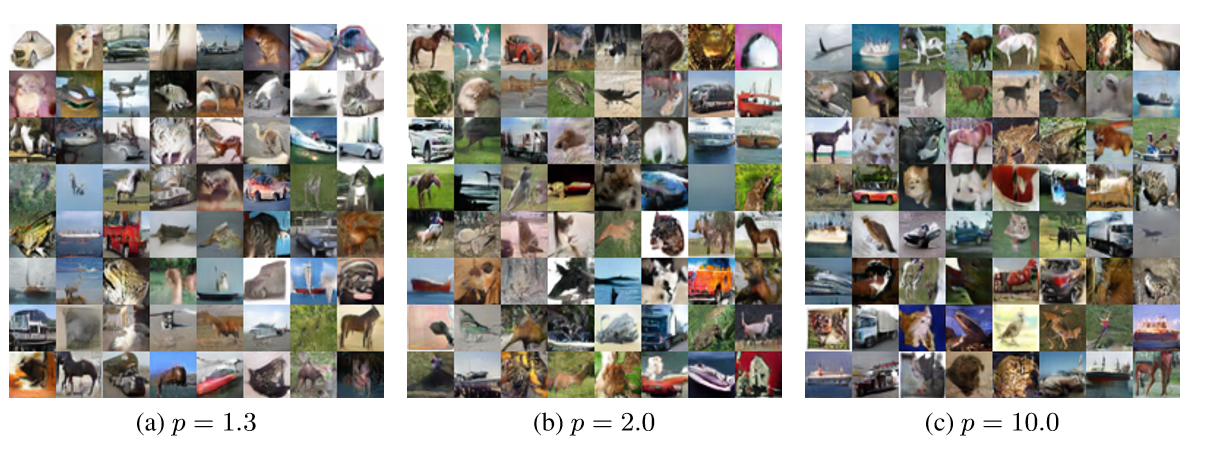
\includegraphics[scale=0.8]{figure/fig1.png}
\caption{Generated CIFAR-10 samples for some $L^p$ spaces.}
\end{figure}

\end{itemize}
\end{flushleft}
\end{frame}

%-----------------------------------------------------------%

\begin{frame}[Computational results]
\begin{flushleft}
\begin{itemize}
\item A high image quality corresponds to \textbf{low} FID scores. \\
\begin{figure}
\center
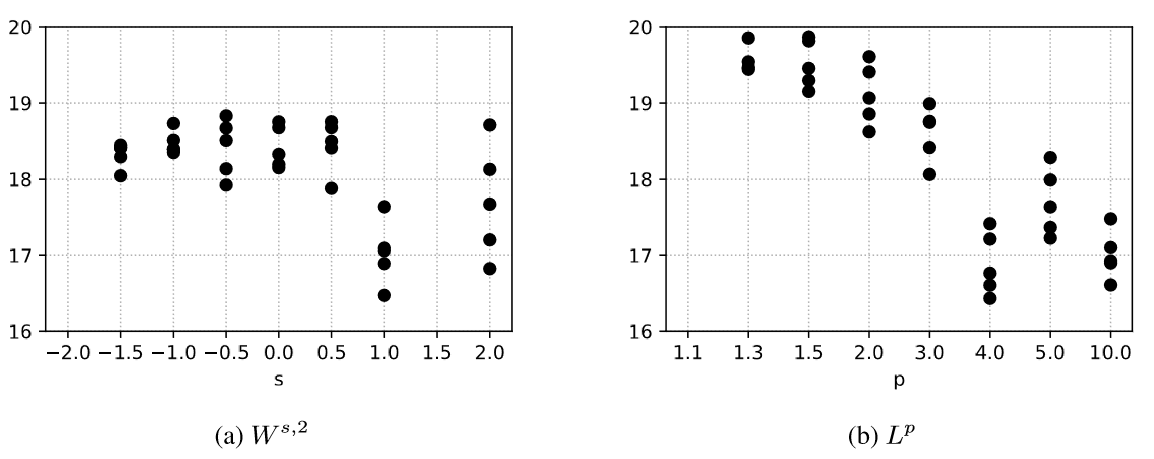
\includegraphics[scale=0.8]{figure/fig2.png}
\caption{FID scores for BWGAN on CIFAR-10.}
\end{figure}

\end{itemize}
\end{flushleft}
\end{frame}

%-----------------------------------------------------------%

\begin{frame}[Computational results]
\begin{flushleft}
\begin{itemize}
\item A high image quality corresponds to \textbf{high} Inception scores. \\
\begin{figure}
\center
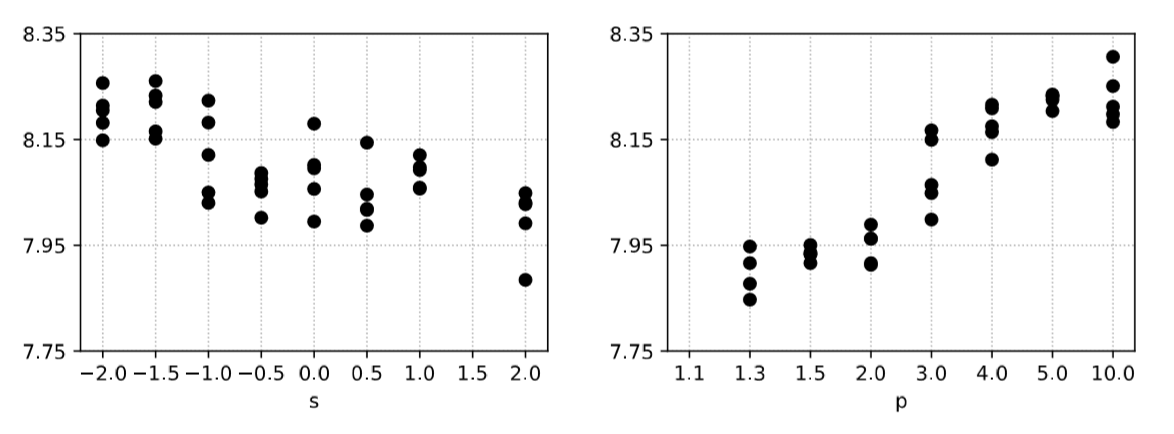
\includegraphics[scale=0.8]{figure/fig3.png}
\caption{Inception scores for BWGAN on CIFAR-10.}
\end{figure}

\end{itemize}
\end{flushleft}
\end{frame}

%-----------------------------------------------------------%

\begin{frame}[Computational results]
\begin{flushleft}
\begin{itemize}
\begin{figure}
\center
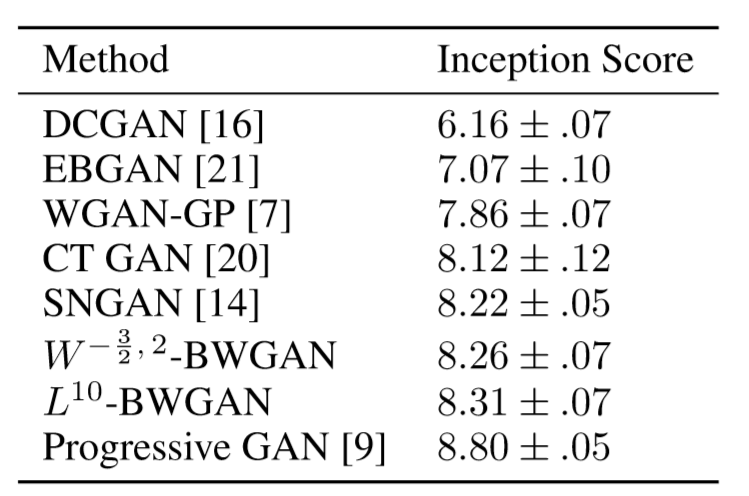
\includegraphics[scale=0.8]{figure/fig4.png}
\caption{Inception scores on CIFAR-10.}
\end{figure}

\end{itemize}
\end{flushleft}
\end{frame}

%-----------------------------------------------------------%

\begin{frame}[Computational results]
\begin{flushleft}
\begin{itemize}
\item Different norm are suitable for different dataset. \\
\begin{figure}
\center
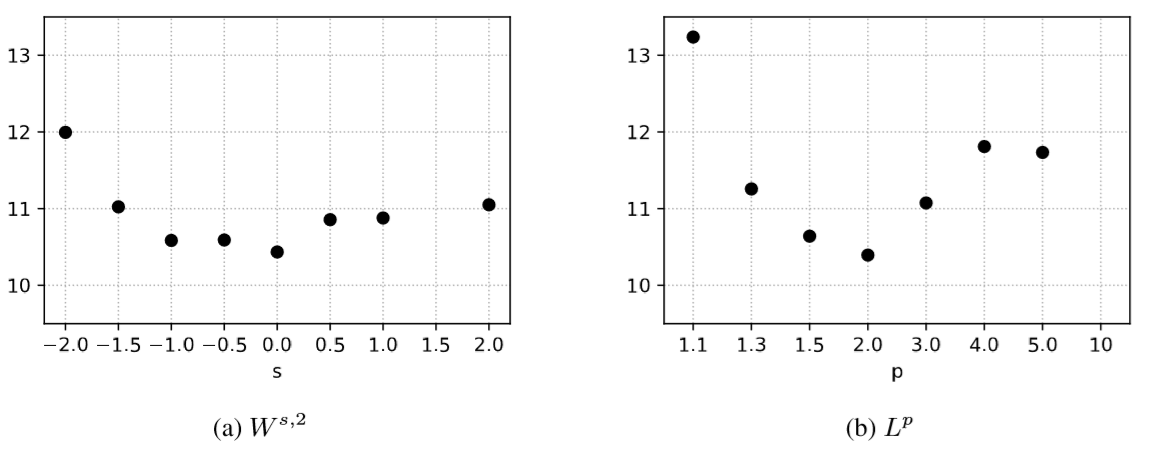
\includegraphics[scale=0.8]{figure/fig6.png}
\caption{FID scores for BWGAN on CelebA.}
\end{figure}

\end{itemize}
\end{flushleft}
\end{frame}

%-----------------------------------------------------------%
%\section{Metric spaces}
%\tableofcontents
%\begin{frame}[Metrics spaces]
%\begin{flushleft}
%\begin{itemize}
%\item Gradient norm penalization according to \textbf{lemma 1} is only valid in Banach spaces. \\
%\item A natural alternativeto penalizing gradient norms is to enforce the Lipschitz condition directly by adding apenalty term of the form
%\begin{equation}
%\mathbb{E}_{X,Y} \left[ \left( \dfrac{|f(x)-f(y)|}{d_B(X,Y)} - 1 \right)^2_+ \right].
%\end{equation}
%\item 
%\end{itemize}
%\end{flushleft}
%\end{frame}

%-----------------------------------------------------------%
\section{Conclusion}
\tableofcontents
\begin{frame}[\secname]
\begin{flushleft}
\begin{itemize}
\item This paper analyzed the dependence of WGANs on the notion of distance between \textbf{images}. \\
\item Showed how choosing distances other than the $\ell^2$ metric can be used to make WGANs focus on \textbf{particular image features} of interest. \\
\item Generalize of WGANs with gradient norm penalization to \textbf{Banach spaces}, allowing to easily implement WGANs for a wide range of underlying norms on images. \\
\item This work was motivated by images, the theory is general and can be applied to data in \textbf{any normed space}.
\end{itemize}
\end{flushleft}
\end{frame}

%\references
%\makethanks

\endslide
\end{document}
